% Options for packages loaded elsewhere
\PassOptionsToPackage{unicode}{hyperref}
\PassOptionsToPackage{hyphens}{url}
\PassOptionsToPackage{dvipsnames,svgnames,x11names}{xcolor}
%
\documentclass[
  a4paper,
]{scrreport}

\usepackage{amsmath,amssymb}
\usepackage{iftex}
\ifPDFTeX
  \usepackage[T1]{fontenc}
  \usepackage[utf8]{inputenc}
  \usepackage{textcomp} % provide euro and other symbols
\else % if luatex or xetex
  \usepackage{unicode-math}
  \defaultfontfeatures{Scale=MatchLowercase}
  \defaultfontfeatures[\rmfamily]{Ligatures=TeX,Scale=1}
\fi
\usepackage{lmodern}
\ifPDFTeX\else  
    % xetex/luatex font selection
\fi
% Use upquote if available, for straight quotes in verbatim environments
\IfFileExists{upquote.sty}{\usepackage{upquote}}{}
\IfFileExists{microtype.sty}{% use microtype if available
  \usepackage[]{microtype}
  \UseMicrotypeSet[protrusion]{basicmath} % disable protrusion for tt fonts
}{}
\makeatletter
\@ifundefined{KOMAClassName}{% if non-KOMA class
  \IfFileExists{parskip.sty}{%
    \usepackage{parskip}
  }{% else
    \setlength{\parindent}{0pt}
    \setlength{\parskip}{6pt plus 2pt minus 1pt}}
}{% if KOMA class
  \KOMAoptions{parskip=half}}
\makeatother
\usepackage{xcolor}
\setlength{\emergencystretch}{3em} % prevent overfull lines
\setcounter{secnumdepth}{5}
% Make \paragraph and \subparagraph free-standing
\ifx\paragraph\undefined\else
  \let\oldparagraph\paragraph
  \renewcommand{\paragraph}[1]{\oldparagraph{#1}\mbox{}}
\fi
\ifx\subparagraph\undefined\else
  \let\oldsubparagraph\subparagraph
  \renewcommand{\subparagraph}[1]{\oldsubparagraph{#1}\mbox{}}
\fi


\providecommand{\tightlist}{%
  \setlength{\itemsep}{0pt}\setlength{\parskip}{0pt}}\usepackage{longtable,booktabs,array}
\usepackage{calc} % for calculating minipage widths
% Correct order of tables after \paragraph or \subparagraph
\usepackage{etoolbox}
\makeatletter
\patchcmd\longtable{\par}{\if@noskipsec\mbox{}\fi\par}{}{}
\makeatother
% Allow footnotes in longtable head/foot
\IfFileExists{footnotehyper.sty}{\usepackage{footnotehyper}}{\usepackage{footnote}}
\makesavenoteenv{longtable}
\usepackage{graphicx}
\makeatletter
\def\maxwidth{\ifdim\Gin@nat@width>\linewidth\linewidth\else\Gin@nat@width\fi}
\def\maxheight{\ifdim\Gin@nat@height>\textheight\textheight\else\Gin@nat@height\fi}
\makeatother
% Scale images if necessary, so that they will not overflow the page
% margins by default, and it is still possible to overwrite the defaults
% using explicit options in \includegraphics[width, height, ...]{}
\setkeys{Gin}{width=\maxwidth,height=\maxheight,keepaspectratio}
% Set default figure placement to htbp
\makeatletter
\def\fps@figure{htbp}
\makeatother

\usepackage{venndiagram}
\newcommand{\NN}{\mathbb{N}}
\newcommand{\ZZ}{\mathbb{Z}}
\newcommand{\QQ}{\mathbb{Q}}
\newcommand{\RR}{\mathbb{R}}
\newcommand{\CC}{\mathbb{C}}
\DeclareMathOperator{\operatorname{Int}}{Int}
\DeclareMathOperator{\operatorname{Ext}}{Ext}
\DeclareMathOperator{\operatorname{Fr}}{Fr}
\DeclareMathOperator{\Adh}{Adh}
\DeclareMathOperator{\Ac}{Ac}
\DeclareMathOperator{\sen}{sen}
\usepackage{booktabs}
\usepackage{longtable}
\usepackage{array}
\usepackage{multirow}
\usepackage{wrapfig}
\usepackage{float}
\usepackage{colortbl}
\usepackage{pdflscape}
\usepackage{tabu}
\usepackage{threeparttable}
\usepackage{threeparttablex}
\usepackage[normalem]{ulem}
\usepackage{makecell}
\usepackage{xcolor}
\makeatletter
\@ifpackageloaded{tcolorbox}{}{\usepackage[skins,breakable]{tcolorbox}}
\@ifpackageloaded{fontawesome5}{}{\usepackage{fontawesome5}}
\definecolor{quarto-callout-color}{HTML}{909090}
\definecolor{quarto-callout-note-color}{HTML}{0758E5}
\definecolor{quarto-callout-important-color}{HTML}{CC1914}
\definecolor{quarto-callout-warning-color}{HTML}{EB9113}
\definecolor{quarto-callout-tip-color}{HTML}{00A047}
\definecolor{quarto-callout-caution-color}{HTML}{FC5300}
\definecolor{quarto-callout-color-frame}{HTML}{acacac}
\definecolor{quarto-callout-note-color-frame}{HTML}{4582ec}
\definecolor{quarto-callout-important-color-frame}{HTML}{d9534f}
\definecolor{quarto-callout-warning-color-frame}{HTML}{f0ad4e}
\definecolor{quarto-callout-tip-color-frame}{HTML}{02b875}
\definecolor{quarto-callout-caution-color-frame}{HTML}{fd7e14}
\makeatother
\makeatletter
\makeatother
\makeatletter
\@ifpackageloaded{bookmark}{}{\usepackage{bookmark}}
\makeatother
\makeatletter
\@ifpackageloaded{caption}{}{\usepackage{caption}}
\AtBeginDocument{%
\ifdefined\contentsname
  \renewcommand*\contentsname{Table of contents}
\else
  \newcommand\contentsname{Table of contents}
\fi
\ifdefined\listfigurename
  \renewcommand*\listfigurename{List of Figures}
\else
  \newcommand\listfigurename{List of Figures}
\fi
\ifdefined\listtablename
  \renewcommand*\listtablename{List of Tables}
\else
  \newcommand\listtablename{List of Tables}
\fi
\ifdefined\figurename
  \renewcommand*\figurename{Figure}
\else
  \newcommand\figurename{Figure}
\fi
\ifdefined\tablename
  \renewcommand*\tablename{Table}
\else
  \newcommand\tablename{Table}
\fi
}
\@ifpackageloaded{float}{}{\usepackage{float}}
\floatstyle{ruled}
\@ifundefined{c@chapter}{\newfloat{codelisting}{h}{lop}}{\newfloat{codelisting}{h}{lop}[chapter]}
\floatname{codelisting}{Listing}
\newcommand*\listoflistings{\listof{codelisting}{List of Listings}}
\usepackage{amsthm}
\theoremstyle{definition}
\newtheorem{exercise}{Exercise}[chapter]
\theoremstyle{remark}
\AtBeginDocument{\renewcommand*{\proofname}{Proof}}
\newtheorem*{remark}{Remark}
\newtheorem*{solution}{Solution}
\makeatother
\makeatletter
\@ifpackageloaded{caption}{}{\usepackage{caption}}
\@ifpackageloaded{subcaption}{}{\usepackage{subcaption}}
\makeatother
\makeatletter
\@ifpackageloaded{tcolorbox}{}{\usepackage[skins,breakable]{tcolorbox}}
\makeatother
\makeatletter
\@ifundefined{shadecolor}{\definecolor{shadecolor}{rgb}{.97, .97, .97}}
\makeatother
\makeatletter
\makeatother
\makeatletter
\makeatother
\ifLuaTeX
\usepackage[bidi=basic]{babel}
\else
\usepackage[bidi=default]{babel}
\fi
\babelprovide[main,import]{english}
% get rid of language-specific shorthands (see #6817):
\let\LanguageShortHands\languageshorthands
\def\languageshorthands#1{}
\ifLuaTeX
  \usepackage{selnolig}  % disable illegal ligatures
\fi
\IfFileExists{bookmark.sty}{\usepackage{bookmark}}{\usepackage{hyperref}}
\IfFileExists{xurl.sty}{\usepackage{xurl}}{} % add URL line breaks if available
\urlstyle{same} % disable monospaced font for URLs
\hypersetup{
  pdftitle={Physiotherapy Statistics Exams},
  pdfauthor={Alfredo Sánchez Alberca},
  pdflang={en},
  colorlinks=true,
  linkcolor={blue},
  filecolor={Maroon},
  citecolor={Blue},
  urlcolor={Blue},
  pdfcreator={LaTeX via pandoc}}

\title{Physiotherapy Statistics Exams}
\author{Alfredo Sánchez Alberca}
\date{2022-01-11}

\begin{document}
\begin{titlepage}

%\AddToShipoutPicture*{\put(0,0){\includegraphics[scale=0.8]{img/background2}}} % Imagen de fondo, requiere el paquete eso-pic.
\begin{center}
\vspace*{5cm}

\Huge
{\textbf{\textsf{Physiotherapy Statistics Exams}}}

\vspace{0.5cm}
\LARGE
{\textbf{\textsf{}}}

\vspace{1.5cm}

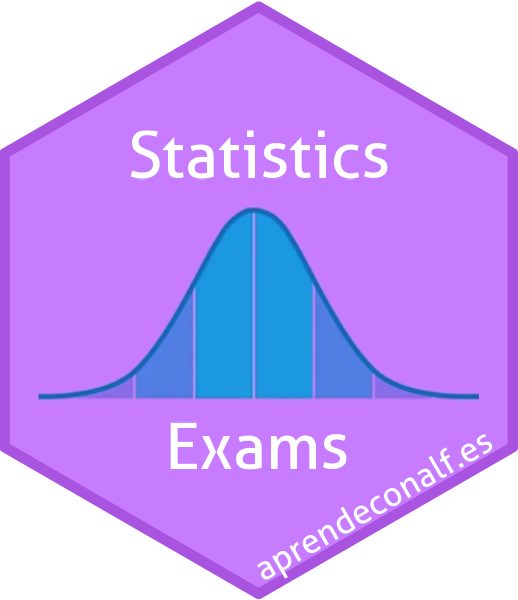
\includegraphics[width=0.4\textwidth]{img/logos/sticker.png}
\end{center}

\vfill

\begin{flushleft}
\begin{tabular}{ll}

\includegraphics[width=0.1\textwidth]{img/logos/aprendeconalf.png} & \parbox[b]{5cm}{\Large\textsf{Alfredo
Sánchez
Alberca}\\ \textsf{asalber@ceu.es} \\ \textsf{https://aprendeconalf.es}}
\end{tabular}
\end{flushleft}
\end{titlepage}\ifdefined\Shaded\renewenvironment{Shaded}{\begin{tcolorbox}[borderline west={3pt}{0pt}{shadecolor}, boxrule=0pt, interior hidden, sharp corners, breakable, enhanced, frame hidden]}{\end{tcolorbox}}\fi

\renewcommand*\contentsname{Table of contents}
{
\hypersetup{linkcolor=}
\setcounter{tocdepth}{2}
\tableofcontents
}
\bookmarksetup{startatroot}

\hypertarget{preface}{%
\chapter*{Preface}\label{preface}}
\addcontentsline{toc}{chapter}{Preface}

\markboth{Preface}{Preface}

Statistics exam collection of the Physiotherapy degree.

\bookmarksetup{startatroot}

\hypertarget{descriptive-statistics-and-regression-exam-20180531}{%
\chapter{Descriptive Statistics and Regression exam
(2018/05/31)}\label{descriptive-statistics-and-regression-exam-20180531}}

\begin{exercise}[]\protect\hypertarget{exr-1}{}\label{exr-1}

~

The ages of a sample of patients of a physical therapy clinic are:

\begin{table}
\centering
\begin{tabular}{r|r|r|r|r|r|r|r|r|r|r|r|r}
\hline
25 & 30 & 44 & 44 & 51 & 51 & 53 & 56 & 57 & 58 & 58 & 58 & 59\\
\hline
59 & 61 & 63 & 63 & 63 & 66 & 68 & 70 & 71 & 72 & 74 & 82 & 85\\
\hline
\end{tabular}
\end{table}

\begin{enumerate}
\def\labelenumi{\alph{enumi}.}
\item
  Compute the quartiles.
\item
  Draw the box plot and identify outliers (do not group data into
  intervals).
\item
  Split the sample into two groups, patients younger and older than 65.
  In which group is the mean more representative. Justify the answer.
\item
  Which distribution is less symmetric, the one of patients younger than
  65 or the one of patients older?
\item
  Which age is relatively smaller with respect to its group, 50 years in
  the group of patients younger than 65 or 72 years in the group of
  patients older than 65?
\end{enumerate}

Use the following sums for the computations.\\
Younger than 65: \(\sum x_i=953\) years, \(\sum x_i^2=52475\)
years\(^2\), \(\sum (x_i-\bar x)^3=-30846.51\) years\(^3\) and
\(\sum (x_i-\bar x)^4=939658.83\) years\(^4\).\\
Older than 65: \(\sum x_i=588\) years, \(\sum x_i^2=43530\) years\(^2\),
\(\sum (x_i-\bar x)^3=1485\) years\(^3\) and
\(\sum (x_i-\bar x)^4=26983.5\) years\(^4\).

\end{exercise}

\begin{tcolorbox}[enhanced jigsaw, toptitle=1mm, leftrule=.75mm, bottomrule=.15mm, coltitle=black, rightrule=.15mm, opacityback=0, breakable, colbacktitle=quarto-callout-tip-color!10!white, bottomtitle=1mm, titlerule=0mm, title=\textcolor{quarto-callout-tip-color}{\faLightbulb}\hspace{0.5em}{Solution}, arc=.35mm, left=2mm, colframe=quarto-callout-tip-color-frame, toprule=.15mm, opacitybacktitle=0.6, colback=white]

\begin{enumerate}
\def\labelenumi{\alph{enumi}.}
\tightlist
\item
  \(Q_1=53\) years, \(Q_2=59\) years and \(Q_3=68\) years.
\item
  There are 2 outliers: 25, 30.
\end{enumerate}

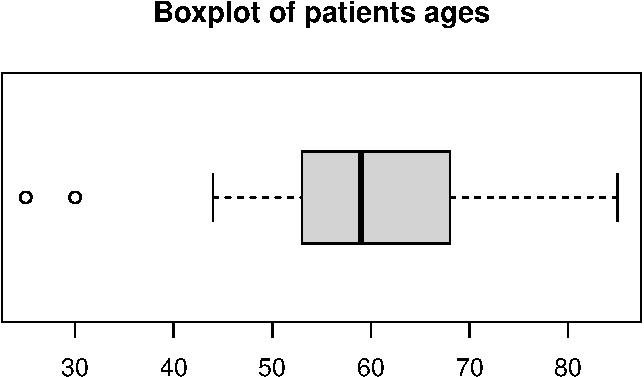
\includegraphics{img/exam-2018-05-31/boxplot-ages-1.pdf}

\begin{enumerate}
\def\labelenumi{\alph{enumi}.}
\item
  Let \(x\) be the age in patients younger than 65 and \(y\) the age in
  patients older than 65.\\
  \(\bar x=52.9444\) years, \(s_x^2=112.1636\) years\(^2\),
  \(s_x=10.5907\) years and \(cv_x=0.2\).\\
  \(\bar y=73.5\) years, \(s_y^2=39\) years\(^2\), \(s_y=6.245\) years
  and \(cv_y=0.085\).\\
  The mean is more representative in patients older than 65 since the
  coefficient of variation is smaller.
\item
  \(g_{1x}=-1.4426\) and \(g_{1y}=0.7621\), thus the distribution of
  ages of people younger than 65 is less symmetric.
\item
  The standard scores are \(z_x(50)=-0.278\) and \(z_y(72)=-0.2402\),
  thus 50 years is relative smaller in the group of people younger than
  65.
\end{enumerate}

\end{tcolorbox}

\begin{exercise}[]\protect\hypertarget{exr-2}{}\label{exr-2}

~

The table below shows the number of injuries of several teams during a
league and the average warm-up time of its players.

\begin{table}
\centering
\begin{tabular}{l|r|r|r|r|r|r|r|r|r|r}
\hline
Warm-up time & 15 & 35 & 22 & 28 & 21 & 18 & 25 & 30 & 23 & 20\\
\hline
Injuries & 42 & 2 & 16 & 6 & 17 & 29 & 10 & 3 & 12 & 20\\
\hline
\end{tabular}
\end{table}

\begin{enumerate}
\def\labelenumi{\alph{enumi}.}
\item
  Draw the scatter plot.
\item
  Which regression model is more suitable to predict the number of
  injuries as a function of the warm-up time, the logarithmic or the
  exponential? Use that regression model to predict the expected number
  of injuries for a team whose players warm-up 20 minutes a day.
\item
  Which regression model is more suitable to predict the warm-up time as
  a function of the number of injuries, the logarithmic or the
  exponential? Use that regression model to predict the warm-up time
  required to have no more than 10 injuries in a league.
\item
  Are these predictions reliable? Which one is more reliable?
\end{enumerate}

Use the following sums for the computations (\(X\) warm-up time and
\(Y\) number of injuries):\\
\(\sum x_i=237\), \(\sum \log(x_i)=31.3728\), \(\sum y_j=157\),
\(\sum \log(y_j)=24.0775\),\\
\(\sum x_i^2=5937\), \(\sum \log(x_i)^2=98.9906\), \(\sum y_j^2=3843\),
\(\sum \log(y_j)^2=66.3721\),\\
\(\sum x_iy_j=3115\), \(\sum x_i\log(y_j)=519.1907\),
\(\sum \log(x_i)y_j=465.8093\), \(\sum \log(x_i)\log(y_j)=73.3995\).

\end{exercise}

\begin{tcolorbox}[enhanced jigsaw, toptitle=1mm, leftrule=.75mm, bottomrule=.15mm, coltitle=black, rightrule=.15mm, opacityback=0, breakable, colbacktitle=quarto-callout-tip-color!10!white, bottomtitle=1mm, titlerule=0mm, title=\textcolor{quarto-callout-tip-color}{\faLightbulb}\hspace{0.5em}{Solution}, arc=.35mm, left=2mm, colframe=quarto-callout-tip-color-frame, toprule=.15mm, opacitybacktitle=0.6, colback=white]

\begin{enumerate}
\def\labelenumi{\alph{enumi}.}
\tightlist
\item
\end{enumerate}

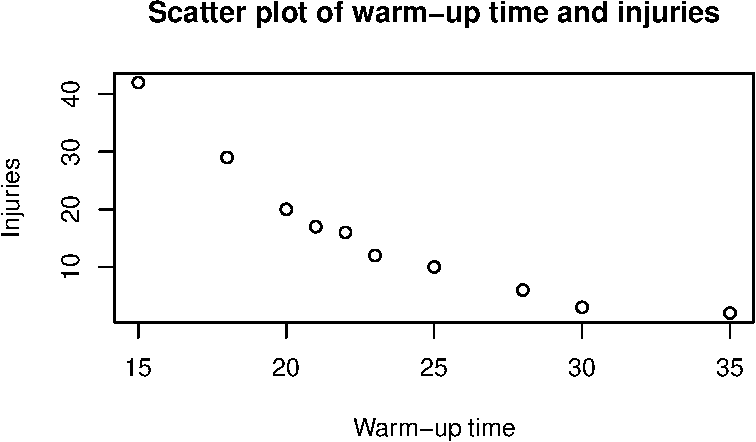
\includegraphics{img/exam2018-05-31/scatterplot-injuries-warm-up-1.pdf}

\begin{enumerate}
\def\labelenumi{\alph{enumi}.}
\item
  \(\bar x=23.7\) min, \(s_x^2=32.01\) min\(^2\).\\
  \(\overline{\log(x)}=3.1373\) log(min), \(s_{\log(x)}^2=0.0565\)
  log(min)\(^2\).\\
  \(\bar y=15.7\) injuries, \(s_y^2=137.81\) injuries\(^2\).\\
  \(\overline{\log(y)}=2.4078\) log(injuries), \(s_{\log(y)}^2=0.8399\)
  log(injuries)\(^2\).\\
  \(s_{x\log(y)}=-5.1446\), \(s_{\log(x)y}=-2.6744\)\\
  Exponential determination coefficient: \(r^2=0.9844\)\\
  Logarithmic determination coefficient: \(r^2=0.9185\)\\
  So the exponential regression model es better to predict the number of
  injuries as a function of the warm-up time.\\
  Exponential regression model: \(y=e^{6.2168+-0.1607x}\).\\
  Prediction: \(y(20)=20.1341\) injuries.
\item
  The logarithmic model is better to predict the warm-up time as a
  function of the number or injuries.\\
  Logarithmic regression model: \(x=164.1851+-47.3292\log(y)\).\\
  Prediction: \(x(10)=55.2056112\) min.
\item
  Both predictions are very reliable since de deternation coefficient is
  very high but the last one is a little less reliable as it is for a
  value further from the data range.
\end{enumerate}

\end{tcolorbox}

\bookmarksetup{startatroot}

\hypertarget{probability-and-random-variables-exam-2022-05-06}{%
\chapter{Probability and Random Variables Exam
(2022-05-06)}\label{probability-and-random-variables-exam-2022-05-06}}

\begin{exercise}[]\protect\hypertarget{exr-1}{}\label{exr-1}

~

8\% of people in a population consume cocaine. It is also known that
4\%: of people who consume cocaine have a heart attack and 10\%: of
people who have a heart attack consume cocaine.

\begin{enumerate}
\def\labelenumi{\alph{enumi}.}
\item
  Construct the probability tree for the random experiment of drawing a
  random person from the population and measuring if he or she consumes
  cocaine and if he or she has a heart attack.
\item
  Compute the probability that a random person of the population does
  not consume cocaine and does not have a heart attack.
\item
  Are the events of consuming cocaine and having a heart attack
  dependent?
\item
  Compute the relative risk and the odds ratio of suffering a heart
  attack consuming cocaine. Which association measure is more suitable
  for this study? Interpret it.
\end{enumerate}

\begin{tcolorbox}[enhanced jigsaw, toptitle=1mm, leftrule=.75mm, bottomrule=.15mm, coltitle=black, rightrule=.15mm, opacityback=0, breakable, colbacktitle=quarto-callout-tip-color!10!white, bottomtitle=1mm, titlerule=0mm, title=\textcolor{quarto-callout-tip-color}{\faLightbulb}\hspace{0.5em}{Solution}, arc=.35mm, left=2mm, colframe=quarto-callout-tip-color-frame, toprule=.15mm, opacitybacktitle=0.6, colback=white]

Let \(C\) the event of consuming cocaine and \(H\) the event of having a
heart attack.

\begin{enumerate}
\def\labelenumi{\alph{enumi}.}
\tightlist
\item
\end{enumerate}

\begin{figure}[H]

{\centering 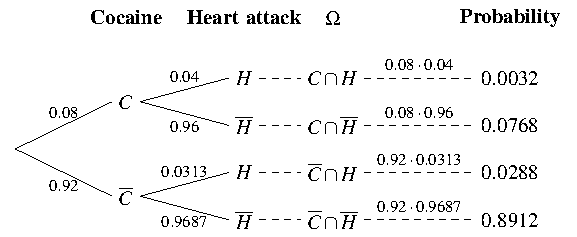
\includegraphics{img/exam-2022-05-06/probability-tree-cocaine.pdf}

}

\caption{Probability tree}

\end{figure}

\begin{enumerate}
\def\labelenumi{\alph{enumi}.}
\item
  \(P(\overline C\cap \overline H)=0.8912\).
\item
  The events are dependent as \(P(C)=0.08\neq P(C|H)=0.1\).
\item
  \(RR(H)=1.2778\) and \(OR(H)=1.2894\). The odds ratio is more suitable
  as the study is retrospective. That means that the odds of having a
  heart attack is \(1.2894\) times greater if a person consumes cocaine.
\end{enumerate}

\end{tcolorbox}

\end{exercise}

\begin{exercise}[]\protect\hypertarget{exr-2}{}\label{exr-2}

~

A basketball player scores 12 points per game on average.

\begin{enumerate}
\def\labelenumi{\alph{enumi}.}
\item
  What is the probability that the player scores more than 4 points in a
  quarter?
\item
  If the player plays 10 games in a league, what is the probability of
  scoring less than 6 points in some game?
\end{enumerate}

\begin{tcolorbox}[enhanced jigsaw, toptitle=1mm, leftrule=.75mm, bottomrule=.15mm, coltitle=black, rightrule=.15mm, opacityback=0, breakable, colbacktitle=quarto-callout-tip-color!10!white, bottomtitle=1mm, titlerule=0mm, title=\textcolor{quarto-callout-tip-color}{\faLightbulb}\hspace{0.5em}{Solution}, arc=.35mm, left=2mm, colframe=quarto-callout-tip-color-frame, toprule=.15mm, opacitybacktitle=0.6, colback=white]

\begin{enumerate}
\def\labelenumi{\alph{enumi}.}
\item
  Let \(X\) be the points scored in a quarter by the player. Then
  \(X\sim P(3)\), and \(P(X>4)=0.1847\).
\item
  Let \(Y\) be the number of points scored in a game by the player. Then
  \(Y\sim P(12)\) and \(P(Y<6)=0.0203\).\\
  Let \(Z\) be the number of games with less than 6 points scored by the
  player. Then \(Z\sim B(10, 0.0203)\), and \(P(Z>0)=0.1858\).
\end{enumerate}

\end{tcolorbox}

\end{exercise}

\begin{exercise}[]\protect\hypertarget{exr-3}{}\label{exr-3}

~

The creatine phosphokinase (CPK3) is an enzyme in the body that causes
the phosphorylation of creatine. This enzyme is found in the skeletal
muscle and can be measured in a blood analysis. The concentration of
CPK3 in blood is normally distributed, and the interval centered at the
mean with the reference values, that accumulates 99\%: of the
population, ranges from 40 to 308 IU/L in healthy adult males.

\begin{enumerate}
\def\labelenumi{\alph{enumi}.}
\item
  Compute the mean and the standard deviation of the concentration of
  CPK3 in healthy males.\\
  Note: If you are not able to compute the standard deviation, use
  \(\sigma = 50\) UI/L for the next parts.
\item
  A diagnostic test to detect muscular dystrophy gives a negative
  outcome when the concentration of CPK3 is below 300 UI/L. Compute the
  specificity of the test.
\item
  If the concentration of CPK3 in people with muscular dystrophy also
  follows a normal distribution with mean 350 IU/L and the same standard
  deviation, what is the sensitivity of the test?
\item
  Compute the predictive values of the test and interpret them assuming
  that the muscular dystrophy prevalence is 8\%.
\end{enumerate}

\begin{tcolorbox}[enhanced jigsaw, toptitle=1mm, leftrule=.75mm, bottomrule=.15mm, coltitle=black, rightrule=.15mm, opacityback=0, breakable, colbacktitle=quarto-callout-tip-color!10!white, bottomtitle=1mm, titlerule=0mm, title=\textcolor{quarto-callout-tip-color}{\faLightbulb}\hspace{0.5em}{Solution}, arc=.35mm, left=2mm, colframe=quarto-callout-tip-color-frame, toprule=.15mm, opacitybacktitle=0.6, colback=white]

\begin{enumerate}
\def\labelenumi{\alph{enumi}.}
\item
  \(\mu = 174\) IU/L and \(\sigma = 51.938\) IU/L.
\item
  Specificity = \(0.9924\).
\item
  Sensitivity = \(0.8321\).\\
  The test is better to confirm the disease as the specificity is
  greater than the sensitivity.
\item
  PPV = \(0.9046\). Thus, we can diagnose the disease with a positive
  outcome.\\
  NPV = \(0.9855\). Thus, we can rule out the disease with a negative
  outcome.
\end{enumerate}

\end{tcolorbox}

\end{exercise}

\bookmarksetup{startatroot}

\hypertarget{descriptive-statistics-and-regression-exam-2022-06-06}{%
\chapter{Descriptive Statistics and Regression Exam
(2022-06-06)}\label{descriptive-statistics-and-regression-exam-2022-06-06}}

\begin{exercise}[]\protect\hypertarget{exr-1}{}\label{exr-1}

~

The patients of a physiotherapy clinic were asked to assess their
satisfaction in a scale from 0 to 10. The assessments are summarized in
the table below.

\[
\begin{array}{lr} 
\hline
\mbox{Assessment} & \mbox{Patients}\\  
0 - 2 & 3\\
2 - 4 & 12\\  
4 - 6 & 9\\ 
6 - 8 & 18\\ 
8 - 10 & 22\\ 
\hline
\end{array}
\]

\begin{enumerate}
\def\labelenumi{\alph{enumi}.}
\item
  Compute the interquartile range of the assessment and interpret it.
\item
  If it is required an assessment greater than 5 in more than 50\%: of
  patients for the clinic to remain open, will the clinic remain open?
\item
  Is the assessment mean representative?
\item
  Compute the coefficient of kurtosis of the assessment and interpret
  it. Is the kurtosis normal?
\item
  If the assessment mean of another clinic is 6.8 and the standard
  deviation is 2.6, which assessment is relatively higher 6 in the first
  clinic or 6.2 in the second?
\end{enumerate}

Use the following sums for the computations:\\
\(\sum x_in_i=408\), \(\sum x_i^2n_i=3000\),
\(\sum (x_i-\bar x)^3n_i=-548.25\) and
\(\sum (x_i-\bar x)^4n_i=5140.45\).

\begin{tcolorbox}[enhanced jigsaw, toptitle=1mm, leftrule=.75mm, bottomrule=.15mm, coltitle=black, rightrule=.15mm, opacityback=0, breakable, colbacktitle=quarto-callout-tip-color!10!white, bottomtitle=1mm, titlerule=0mm, title=\textcolor{quarto-callout-tip-color}{\faLightbulb}\hspace{0.5em}{Solution}, arc=.35mm, left=2mm, colframe=quarto-callout-tip-color-frame, toprule=.15mm, opacitybacktitle=0.6, colback=white]

Let \(X\) be the patient assessment. a. \(Q_1= 4.4444\), \(Q_3=9.0907\)
and \(IQR = 4.6463\), so the central dispersion is moderate.

\begin{enumerate}
\def\labelenumi{\alph{enumi}.}
\item
  \(F(5)=0.2695\), and the percentage of patients with an assessment
  greater than 5 is \(73.05%:
  \).
\item
  \(\bar x = 6.375\), \(s_x^2 = 6.2344\), \(s_x=2.4969\) and
  \(cv=0.3917\), thus the representativity of the mean is moderate.
\item
  \(g_2 = -0.9335\) and the distribution is flatter than a Gauss bell,
  but normal, as \(g_2\) is between -2 and 2.
\item
  First clinic: \(z(6)=-0.1502\)\\
  Second clinic: \(z(6.2)=-0.3077\).\\
  Thus, an assessment of 6 in the first clinic is relatively higher as
  its standard score is greater.
\end{enumerate}

\end{tcolorbox}

\end{exercise}

\begin{exercise}[]\protect\hypertarget{exr-2}{}\label{exr-2}

~

A study tries to determine the effectiveness a training program to
increase the grip strength. The table below shows the grip strength in
Kg in some weeks of the training program.

\begin{table}
\centering
\begin{tabular}{l|r|r|r|r|r|r|r|r}
\hline
Week & 1 & 3 & 6 & 9 & 14 & 17 & 21 & 24\\
\hline
Grip strength & 15 & 22 & 29 & 34 & 36 & 39 & 40 & 41\\
\hline
\end{tabular}
\end{table}

\begin{enumerate}
\def\labelenumi{\alph{enumi}.}
\item
  Compute the regression coefficient of the grip strength on the weeks
  and interpret it.
\item
  According to the logarithmic regression model, what is the expected
  grip strength after 5 and 25 weeks. Are these predictions reliable?
  Would these predictions be more reliable with the linear regression
  model?
\item
  According to the exponential regression model, how many weeks are
  required to have a grip strength of 25 Kg?
\item
  What percentage of the total variability of the weeks is explained by
  the exponential model?
\end{enumerate}

Use the following sums (\(X\)=Weeks and \(Y\)=Grip strength):\\
\(\sum x_i=95\), \(\sum \log(x_i)=16.7824\), \(\sum y_j=256\),
\(\sum \log(y_j)=27.3423\),\\
\(\sum x_i^2=1629\), \(\sum \log(x_i)^2=43.606\), \(\sum y_j^2=8804\),
\(\sum \log(y_j)^2=94.3237\),\\
\(\sum x_iy_j=3552\), \(\sum x_i\log(y_j)=342.9642\),
\(\sum \log(x_i)y_j=608.4186\), \(\sum \log(x_i)\log(y_j)=60.047\).

\begin{tcolorbox}[enhanced jigsaw, toptitle=1mm, leftrule=.75mm, bottomrule=.15mm, coltitle=black, rightrule=.15mm, opacityback=0, breakable, colbacktitle=quarto-callout-tip-color!10!white, bottomtitle=1mm, titlerule=0mm, title=\textcolor{quarto-callout-tip-color}{\faLightbulb}\hspace{0.5em}{Solution}, arc=.35mm, left=2mm, colframe=quarto-callout-tip-color-frame, toprule=.15mm, opacitybacktitle=0.6, colback=white]

\begin{enumerate}
\def\labelenumi{\alph{enumi}.}
\item
  \(\overline{x}=11.875\) weeks, \(s_x^2=62.6094\) weeks\(^2\).\\
  \(\bar y=32\) Kg, \(s_y^2=76.5\) Kg\(^2\).\\
  \(s_{xy}=64\) weeks\(\cdot\)Kg.\\
  Regression coefficient of \(Y\) on \(X\): \(b_{yx} = 1.0222\)
  Kg/weeek. The grip strength increases \(1.0222\) Kg per week.
\item
  \(\overline{\ln(x)} = 2.0978\) ln(weeks), \(s_{\ln(x)}^2 = 1.05\)
  ln(weeks)\(^2\) and \(s_{\ln(x)y} = 8.9226\) ln(weeks)Kg.\\
  Logarithmic regression model of \(Y\) on \(X\):
  \(y = 14.1729 + 8.498 \ln(x)\).\\
  Predictions: \(y(5) = 27.8499\) Kg and \(y(25) = 41.5268\) Kg.\\
  Logarithmic coefficient of determination: \(r^2 = 0.9912\). The
  predictions are not reliable because the sample size is small.\\
  Linear coefficient of determination: \(r^2 = 0.8552\).\\
  As the linear coefficient of determination is less than the
  logarithmic one, the predictions with the logarithmic model are more
  reliable.
\item
  Exponential regression model of \(X\) on \(Y\):
  \(x = e^{-1.6345 + 0.1166y}\).\\
  Prediction: \(x(25)=3.6015\) Weeks.
\item
  As \(r^2 = 0.9912\), the exponential models explains \(99.12\)\%: of
  the variability of the weeks.\\
\end{enumerate}

\end{tcolorbox}

\end{exercise}

\bookmarksetup{startatroot}

\hypertarget{probability-and-random-variables-exam-2022-06-06}{%
\chapter{Probability and Random Variables Exam
(2022-06-06)}\label{probability-and-random-variables-exam-2022-06-06}}

\begin{exercise}[]\protect\hypertarget{exr-1}{}\label{exr-1}

~

A diagnostic test for a cervical injury has a 99\% of sensitivity and
produces 80\% of right diagnosis. Assuming that the prevalence of the
injury is 10\%

\begin{enumerate}
\def\labelenumi{\alph{enumi}.}
\item
  Compute the specificity of the test.
\item
  Can we rule out the injury with a negative outcome of the test?
\item
  Can we diagnose the injury with a positive outcome of the test? What
  must the minimum prevalence of the injury be to diagnose the injury
  with a positive outcome of the test?
\end{enumerate}

\begin{tcolorbox}[enhanced jigsaw, toptitle=1mm, leftrule=.75mm, bottomrule=.15mm, coltitle=black, rightrule=.15mm, opacityback=0, breakable, colbacktitle=quarto-callout-tip-color!10!white, bottomtitle=1mm, titlerule=0mm, title=\textcolor{quarto-callout-tip-color}{\faLightbulb}\hspace{0.5em}{Solution}, arc=.35mm, left=2mm, colframe=quarto-callout-tip-color-frame, toprule=.15mm, opacitybacktitle=0.6, colback=white]

\begin{enumerate}
\def\labelenumi{\alph{enumi}.}
\item
  Specificity = \(P(-|\overline D) = 0.7789\).
\item
  Negative predictive value = \(P(\overline D|-) = 0.9986 > 0.5\), so we
  can rule out the injury with a negative outcome.
\item
  Positive predictive value = \(P(D|+) = 0.3322 < 0.5\), so we can not
  diagnose the injury with a positive outcome. The minimum prevalence
  required to be able to diagnose the injury with a positive outcome is
  \(P(D)=0.1825\).
\end{enumerate}

\end{tcolorbox}

\end{exercise}

\begin{exercise}[]\protect\hypertarget{exr-2}{}\label{exr-2}

~

A pharmacy sells two vaccines \(A\) and \(B\) against a virus. The \(A\)
vaccine produces 5\%: of side effects, while the \(B\) vaccine produces
2\%: of side effects. The pharmacy has sold 10 units of the \(A\)
vaccine and 100 units of the \(B\) vaccine.

\begin{enumerate}
\def\labelenumi{\alph{enumi}.}
\item
  Compute the probability of having less than 2 side effects with the
  \(A\) vaccine.
\item
  Compute the probability of having more than 3 side effects with the
  \(B\) vaccine.
\item
  If we apply both vaccines to the same person at different moments, and
  assuming that the production of side effects of the vaccines are
  independent, what is the probability that this person will have any
  side effect?
\end{enumerate}

\begin{tcolorbox}[enhanced jigsaw, toptitle=1mm, leftrule=.75mm, bottomrule=.15mm, coltitle=black, rightrule=.15mm, opacityback=0, breakable, colbacktitle=quarto-callout-tip-color!10!white, bottomtitle=1mm, titlerule=0mm, title=\textcolor{quarto-callout-tip-color}{\faLightbulb}\hspace{0.5em}{Solution}, arc=.35mm, left=2mm, colframe=quarto-callout-tip-color-frame, toprule=.15mm, opacitybacktitle=0.6, colback=white]

\begin{enumerate}
\def\labelenumi{\alph{enumi}.}
\item
  Let \(X\) be the number of side effects in 10 applications of A
  vaccine. Then, \(X\sim B(10, 0.05)\) and \(P(X<2) = 0.9139\).
\item
  Let \(Y\) be the number of side effects in 100 applications of B
  vaccine. Then, \(Y\sim B(100, 0.02)\approx P(2)\) and
  \(P(Y>3) = 0.1429\).
\item
  Let \(A\) and \(B\) the events of having side effects with vaccines A
  and B respectively. \(P(A\cup B) = 0.069\).
\end{enumerate}

\end{tcolorbox}

\end{exercise}

\begin{exercise}[]\protect\hypertarget{exr-3}{}\label{exr-3}

~

The length of the femur bone is normally distributed in both men and
women with a standard deviation of 4 cm. It is also known that the first
quartile in women is 42.3 cm, while the third quartile in men is 50.7
cm.

\begin{enumerate}
\def\labelenumi{\alph{enumi}.}
\item
  What is the difference between the means of the femur length of women
  and men?\\
  Remark: If you do not know how to compute the means, use a mean 44 cm
  for women and a mean 47 cm for men in the following parts.
\item
  Compute the 60th percentile of the femur length in women. What
  percentage of men have a femur length less than the 60th percentile of
  women?
\item
  If we pick a woman and man at random, what is the probability that
  neither of them has a femur length less than 45 cm?
\end{enumerate}

\begin{tcolorbox}[enhanced jigsaw, toptitle=1mm, leftrule=.75mm, bottomrule=.15mm, coltitle=black, rightrule=.15mm, opacityback=0, breakable, colbacktitle=quarto-callout-tip-color!10!white, bottomtitle=1mm, titlerule=0mm, title=\textcolor{quarto-callout-tip-color}{\faLightbulb}\hspace{0.5em}{Solution}, arc=.35mm, left=2mm, colframe=quarto-callout-tip-color-frame, toprule=.15mm, opacitybacktitle=0.6, colback=white]

Let \(X\) and \(Y\) be the femur length of women and men respectively.
Then \(X\sim N(\mu_x, 4)\) and \(Y\sim N(\mu_y,4)\).

\begin{enumerate}
\def\labelenumi{\alph{enumi}.}
\item
  \(\mu_x = 44.91\) cm and \(\mu_y = 48.02\) cm.
\item
  60th percentile in women \(P_{60}=45.9234\) cm, and
  \(P(Y<45.9234) = 0.3001\), that is, a \(30.01%:
  \) of men have a femur lenght less than the 60th percentile of women.
\item
  \(P(X\geq 45 \cap Y\geq45) = 0.3805\).
\end{enumerate}

\end{tcolorbox}

\end{exercise}

\bookmarksetup{startatroot}

\hypertarget{descriptive-statistics-and-regression-exam-20230323}{%
\chapter{Descriptive Statistics and Regression exam
(2023/03/23)}\label{descriptive-statistics-and-regression-exam-20230323}}

\begin{exercise}[]\protect\hypertarget{exr-1}{}\label{exr-1}

~

The chart below shows the percentage of grades in a Statistic course
with 60 students.

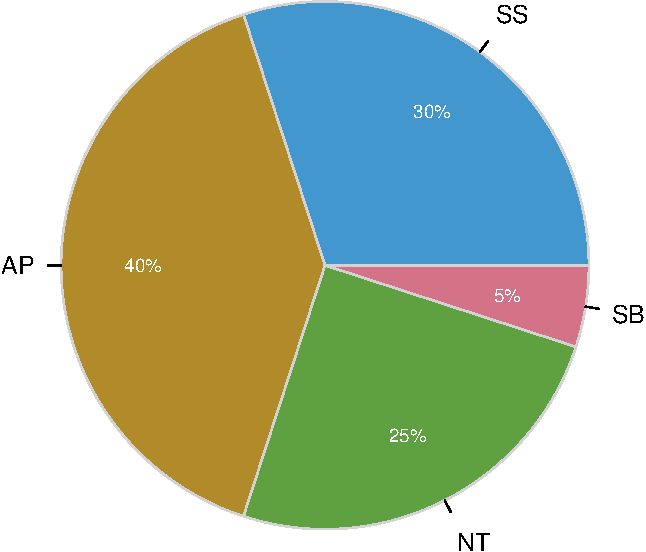
\includegraphics{img/exam-2023-03-23/pie-chart-scores-1.pdf}

\begin{enumerate}
\def\labelenumi{\alph{enumi}.}
\tightlist
\item
  Plot the ogive of the score, assuming the following correspondence
  between grades and scores
\end{enumerate}

\[
\begin{array}{lc}
  \mbox{Grade} & \mbox{Score}\\
  \mbox{SS} & [0, 5)\\
  \mbox{AP} & [5, 7)\\
  \mbox{NT} & [7,9)\\
  \mbox{SB} & [9,10]
\end{array}
\]

\begin{enumerate}
\def\labelenumi{\alph{enumi}.}
\item
  Compute the median and interpret it.
\item
  How many students got a score greater than 8?
\item
  Study the dispersion of the distribution.
\item
  Study the skewness of the distribution. Is it normal?
\item
  If we apply the transformation \(y=10x+5\) to the scores, how changes
  the representativeness of the mean. And the skewness?
\end{enumerate}

Use the following sums for the computations (\(X\) = Score):\\
\(\sum x_in_i=337.5\), \(\sum x_i^2n_i=2207.25\),
\(\sum (x_i-\bar x)^3n_i=-172.55\) and
\(\sum (x_i-\bar x)^4n_i=2870.75\).

\begin{tcolorbox}[enhanced jigsaw, toptitle=1mm, leftrule=.75mm, bottomrule=.15mm, coltitle=black, rightrule=.15mm, opacityback=0, breakable, colbacktitle=quarto-callout-tip-color!10!white, bottomtitle=1mm, titlerule=0mm, title=\textcolor{quarto-callout-tip-color}{\faLightbulb}\hspace{0.5em}{Solution}, arc=.35mm, left=2mm, colframe=quarto-callout-tip-color-frame, toprule=.15mm, opacitybacktitle=0.6, colback=white]

\begin{enumerate}
\def\labelenumi{\alph{enumi}.}
\tightlist
\item
  Ogive
\end{enumerate}

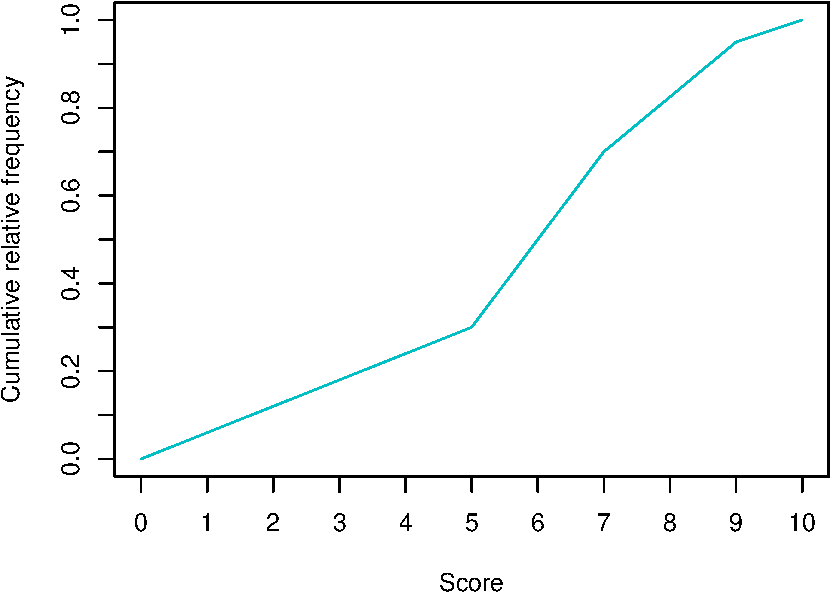
\includegraphics{img/exam-2023-03-23/ogive-scores-1.pdf}

\begin{enumerate}
\def\labelenumi{\alph{enumi}.}
\setcounter{enumi}{1}
\item
  \(Me = 6\) points.
\item
  \(N(8) = 49.5\) students.
\item
  \(\bar x = 5.625\) points, \(s_x^2=5.1469\) points\(^2\),
  \(s_x=2.2687\) points and \(cv_x=0.4033\). Thus, there is a moderate
  dispersion with respect to the mean.
\item
  \(g_1 = -0.2463\) and therefore the distribution is a little bit left
  skewed.
\item
  \(\bar y = 61.25\) points, \(s_y^2=514.6875\) points\(^2\),
  \(s_y=22.6867\) points and \(cv_y=0.3704\). As \(cv_y < cv_x\) the
  representativeness of the mean increases. As the slope of the linear
  transformation is positive, the skewness does not change.
\end{enumerate}

\end{tcolorbox}

\end{exercise}

\begin{exercise}[]\protect\hypertarget{exr-2}{}\label{exr-2}

~

A study tries to determine if there is a relation between the gestation
time (in weeks) and the age of the mother (in years). A sample of 40
mothers was taken and the sums below summarize the results (\(X\)=Age
and \(Y\)=Gestation time):

\(\sum x_i=1262\) years, \(\sum \log(x_i)=137.0078\) log(years),
\(\sum y_j=1583.6\) weeks, \(\sum \log(y_j)=147.1305\) log(weeks),\\
\(\sum x_i^2=41862\) years\(^2\), \(\sum \log(x_i)^2=471.4222\)
log(years)\(^2\), \(\sum y_j^2=62734.685\) weeks\(^2\),
\(\sum \log(y_j)^2=541.2096\) log(weeks)\(^2\),\\
\(\sum x_iy_j=50116.7\) years\(\cdot\)weeks,
\(\sum x_i\log(y_j)=4645.8\) years\(\cdot\)log(weeks),
\(\sum \log(x_i)y_j=5428.9192\) log(years)\(\cdot\)weeks,
\(\sum \log(x_i)\log(y_j)=504.0696\) log(years)\(\cdot\)log(weeks).

\begin{enumerate}
\def\labelenumi{\alph{enumi}.}
\item
  Which regression models, linear, exponential or logarithmic, explains
  better the relation between the age and the gestation time?
\item
  Use the best model to predict the gestation time for a mother 45 years
  old. Is this prediction reliable?
\item
  According to the linear model, how much increases or decreases the
  gestation time for every year of the mother?
\end{enumerate}

\begin{tcolorbox}[enhanced jigsaw, toptitle=1mm, leftrule=.75mm, bottomrule=.15mm, coltitle=black, rightrule=.15mm, opacityback=0, breakable, colbacktitle=quarto-callout-tip-color!10!white, bottomtitle=1mm, titlerule=0mm, title=\textcolor{quarto-callout-tip-color}{\faLightbulb}\hspace{0.5em}{Solution}, arc=.35mm, left=2mm, colframe=quarto-callout-tip-color-frame, toprule=.15mm, opacitybacktitle=0.6, colback=white]

\begin{enumerate}
\def\labelenumi{\alph{enumi}.}
\item
  Linear model: \(\overline{x}=31.55\) years, \(s_x^2=51.1475\)
  years\(^2\).\\
  \(\bar y=39.59\) weeks, \(s_y^2=0.999\) weeks\(^2\).\\
  \(s_{xy}=3.853\) years\(\cdot\)weeks.\\
  \(r^2 = 0.2905\).

  Exponential model: \(\overline{\ln(y)} = 3.6783\) ln(weeks),
  \(s_{\ln(y)}^2 = 0.0006\) ln(weeks)\(^2\)\\
  \(s_{x\ln(y)} = 0.0958\) years\(\cdot\ln\)(weeks).\\
  \(r^2 = 0.2882\).

  Logarithmic model: \(\overline{\ln(x)} = 3.4252\) ln(years),
  \(s_{\ln(x)}^2 = 0.0536\) ln(years)\(^2\)\\
  \(s_{\ln(x)y} = 0.1195\) ln(years)weeks.\\
  \(r^2 = 0.2668\).

  As the linear coefficient of determination is greater, the linear
  model explains better the relation between de gestation time and the
  age of the mother.
\item
  Linear regression model of \(Y\) on \(X\):
  \(y = 37.2133 + 0.0753 x\).\\
  Predictions: \(y(45) = 40.6032\) weeks.\\
  The predictions are not reliable because the coefficient of
  determination is pretty low.
\item
  Regression coefficient of \(Y\) on \(X\): \(b_{yx} = 0.0753\)
  weeks/year. The gestation time increases \(0.0753\) weeks per year.
\end{enumerate}

\end{tcolorbox}

\end{exercise}

\bookmarksetup{startatroot}

\hypertarget{probability-and-random-variables-exam-2023-04-27}{%
\chapter{Probability and Random Variables Exam
(2023-04-27)}\label{probability-and-random-variables-exam-2023-04-27}}

\begin{exercise}[]\protect\hypertarget{exr-1}{}\label{exr-1}

~

A water source contaminated contains 0.1 amoebas per litre on average.

\begin{enumerate}
\def\labelenumi{\alph{enumi}.}
\item
  What is the probability that 2 litres of water from this source
  contains more than one amoeba?
\item
  If 5 persons drink 2 litres of water from this source, what is the
  probability of having some person infected with amoebas?
\item
  If 100 persons drink half a litre of water from this source, what is
  the probability that less than 5 are infected with amoebas?
\end{enumerate}

\begin{tcolorbox}[enhanced jigsaw, toptitle=1mm, leftrule=.75mm, bottomrule=.15mm, coltitle=black, rightrule=.15mm, opacityback=0, breakable, colbacktitle=quarto-callout-tip-color!10!white, bottomtitle=1mm, titlerule=0mm, title=\textcolor{quarto-callout-tip-color}{\faLightbulb}\hspace{0.5em}{Solution}, arc=.35mm, left=2mm, colframe=quarto-callout-tip-color-frame, toprule=.15mm, opacitybacktitle=0.6, colback=white]

\begin{enumerate}
\def\labelenumi{\alph{enumi}.}
\item
  Let \(X\) be the number of amoebas in 2 litres of contaminated water.
  Then \(X\sim P(0.2)\) and \(P(X>1)=0.0175\).
\item
  The probability that a person who drank 2 litres of contaminated water
  is infected is \(P(X\geq 1) = 0.1813\). Let \(Y\) be the number of
  persons infected with amoebas in a sample of 5 persons who drank 2
  litres of contaminated water. Then \(Y\sim B(5, 0.1813)\) and
  \(P(Y\geq 1)=0.6321\).
\item
  Let \(U\) be the number of amoebas in half a litre of contaminated
  water. Then \(U\sim P(0.05)\) and \(P(U\geq 1)= 0.0488\). Let \(V\) be
  the number of persons infected with amoebas in a sample of 100 persons
  who drank half a litre of contaminated water. Then
  \(V\sim B(100, 0.0488)\approx P(4.8771)\) and \(P(V<5) = 0.4623\).
\end{enumerate}

\end{tcolorbox}

\end{exercise}

\begin{exercise}[]\protect\hypertarget{exr-2}{}\label{exr-2}

~

Respiratory allergies affect 1 out of every 15 individuals in a
population, while food intolerances affect 5\% of individuals. Assuming
that the two problems are independent,

\begin{enumerate}
\def\labelenumi{\alph{enumi}.}
\item
  Compute the probability of having at least one of the problems.
\item
  Compute the probability of having an allergy but not an intolerance.
\item
  Compute the probability of having neither of the two problems.
\item
  Compute the probability of having an allergy if you have an
  intolerance.
\end{enumerate}

\begin{tcolorbox}[enhanced jigsaw, toptitle=1mm, leftrule=.75mm, bottomrule=.15mm, coltitle=black, rightrule=.15mm, opacityback=0, breakable, colbacktitle=quarto-callout-tip-color!10!white, bottomtitle=1mm, titlerule=0mm, title=\textcolor{quarto-callout-tip-color}{\faLightbulb}\hspace{0.5em}{Solution}, arc=.35mm, left=2mm, colframe=quarto-callout-tip-color-frame, toprule=.15mm, opacitybacktitle=0.6, colback=white]

Let \(A\) the event of having respiratory allergies and \(B\) the event
of having food intolerance.

\begin{enumerate}
\def\labelenumi{\alph{enumi}.}
\item
  \(P(A\cup B) = 0.1133\).
\item
  \(P(A-B) = 0.0633\).
\item
  \(P(\overline A \cap \overline B) = 0.8867\).
\item
  \(P(A|B) = 0.0667\).
\end{enumerate}

\end{tcolorbox}

\end{exercise}

\begin{exercise}[]\protect\hypertarget{exr-3}{}\label{exr-3}

~

In a population of 20000 women, it is known that back width follows a
normal distribution with mean 29 cm and standard deviation 2.4 cm.

\begin{enumerate}
\def\labelenumi{\alph{enumi}.}
\item
  Compute the number of women with a back width greater than 32 cm.
\item
  Compute the interquartile range of women's back width and interpret
  it.
\item
  Compute the probability that a woman with a back width above the third
  quartile, has a back width above 32.
\end{enumerate}

\begin{tcolorbox}[enhanced jigsaw, toptitle=1mm, leftrule=.75mm, bottomrule=.15mm, coltitle=black, rightrule=.15mm, opacityback=0, breakable, colbacktitle=quarto-callout-tip-color!10!white, bottomtitle=1mm, titlerule=0mm, title=\textcolor{quarto-callout-tip-color}{\faLightbulb}\hspace{0.5em}{Solution}, arc=.35mm, left=2mm, colframe=quarto-callout-tip-color-frame, toprule=.15mm, opacitybacktitle=0.6, colback=white]

Let \(X\) be the back width, then \(X\sim N(29, 2.4)\).

\begin{enumerate}
\def\labelenumi{\alph{enumi}.}
\item
  \(P(X>32) = 0.1056\) and approximately \(2113\) persons have a back
  width greater than 32 cm.
\item
  \(Q_1 = 27.3812\) cm, \(Q_3 = 30.6188\) cm, and \(IQR = 3.2376\) cm.
\item
  \(P(X>32| X>30.6188) = 0.4226\).
\end{enumerate}

\end{tcolorbox}

\end{exercise}

\begin{exercise}[]\protect\hypertarget{exr-4}{}\label{exr-4}

~

A diagnostic test for prostate cancer has a specificity of 80\% and
produces 1.6\% of false negatives. It is known that the prevalence of
prostate cancer in a population is 2\%.

\begin{enumerate}
\def\labelenumi{\alph{enumi}.}
\item
  Compute the sensitivity of the test. Does the outcome of the test
  depend on whether a man has prostate cancer?
\item
  Is this a good test to diagnose the disease?
\item
  What should be the minimum specificity of the test to diagnose the
  disease with a positive outcome?
\end{enumerate}

\begin{tcolorbox}[enhanced jigsaw, toptitle=1mm, leftrule=.75mm, bottomrule=.15mm, coltitle=black, rightrule=.15mm, opacityback=0, breakable, colbacktitle=quarto-callout-tip-color!10!white, bottomtitle=1mm, titlerule=0mm, title=\textcolor{quarto-callout-tip-color}{\faLightbulb}\hspace{0.5em}{Solution}, arc=.35mm, left=2mm, colframe=quarto-callout-tip-color-frame, toprule=.15mm, opacitybacktitle=0.6, colback=white]

\begin{enumerate}
\def\labelenumi{\alph{enumi}.}
\item
  Sensitivity = \(P(+|D) = 0.2\). The outcome of the test does not
  depend on the prostate cancer.
\item
  Positive predictive value = \(P(D|+) = 0.02 < 0.5\), so we can not
  confirm the prostate cancer with a positive outcome.
\item
  Minimum specificity \(0.9959\).
\end{enumerate}

\end{tcolorbox}

\end{exercise}



\end{document}
